% =============================================================================
% Fig 2: OrbitVLIF module zoom-ins
%   (a) 5QS — 5-level quantized spike activation + surrogate gradient
%   (b) MFRB — multi-frequency residual block (dual-path schematic)
%   (c) SHAM — spectral-hybrid attention module (temporal + DCT spatial)
%
% Compile:
%   pdflatex fig2_modules.tex
%
% Style guidelines (kept consistent with fig1.tex):
%   * STIX maths font (Times-like, IEEE recommended)
%   * Wong-2011 colour-blind safe palette
%   * Vector-only, 0.4-0.6 pt strokes, Stealth arrows 4×3 pt
%   * Sub-panel labels (a)(b)(c) bold sans-serif
% =============================================================================
\documentclass[border=4pt, tikz]{standalone}

\usepackage[T1]{fontenc}
\usepackage{stix}
\usepackage{amsmath, amssymb, bm}
\usepackage{tikz}
\usetikzlibrary{
    positioning, arrows.meta, shapes.geometric, calc,
    decorations.pathreplacing, decorations.markings,
    patterns, patterns.meta, fit, backgrounds, shadows
}

% ---- Wong-2011 palette ------------------------------------------------------
\definecolor{cBlue}  {HTML}{0173B2}
\definecolor{cOrange}{HTML}{DE8F05}
\definecolor{cGreen} {HTML}{029E73}
\definecolor{cRed}   {HTML}{D55E00}
\definecolor{cPurple}{HTML}{CC78BC}
\definecolor{cYellow}{HTML}{ECE133}
\definecolor{cGray}  {HTML}{4D4D4D}
\definecolor{cLight} {HTML}{E8E8E8}

% ---- Style helpers ----------------------------------------------------------
\tikzset{
  font=\sffamily\footnotesize,
  >={Stealth[length=4pt, width=3pt]},
  every node/.style={inner sep=2pt, outer sep=0pt, align=center},
  panellbl/.style={font=\sffamily\bfseries\small, text=black},
  arrow/.style={->, line width=0.6pt, draw=cGray, shorten >=1pt, shorten <=1pt},
  thinarrow/.style={->, line width=0.4pt, draw=cGray, shorten >=1pt},
  axis/.style={->, line width=0.6pt, draw=black},
  label/.style={font=\sffamily\scriptsize, text=cGray},
  block/.style={
    rectangle, rounded corners=1.2pt, draw=cGray, line width=0.4pt,
    minimum width=10mm, minimum height=5mm, font=\sffamily\scriptsize,
  },
  lifblk/.style={block, fill=cYellow!35, draw=cOrange!80, font=\sffamily\scriptsize\bfseries},
  convblk/.style={block, fill=cBlue!18, draw=cBlue!70},
  bnblk/.style={block, fill=cGreen!18, draw=cGreen!70, minimum width=8mm},
  gateblk/.style={
    circle, draw=cPurple!80, line width=0.5pt, fill=cPurple!22,
    minimum size=4mm, inner sep=0pt, font=\sffamily\scriptsize,
  },
  cube/.style={draw=cGray, line width=0.35pt},
  spikemark/.pic={
    \draw[line width=0.5pt, draw=cOrange]
      (-0.4mm,1.0mm) -- (0.0mm,-0.2mm) -- (-0.2mm,-0.2mm) -- (0.4mm,-1.0mm);
  },
}

\begin{document}
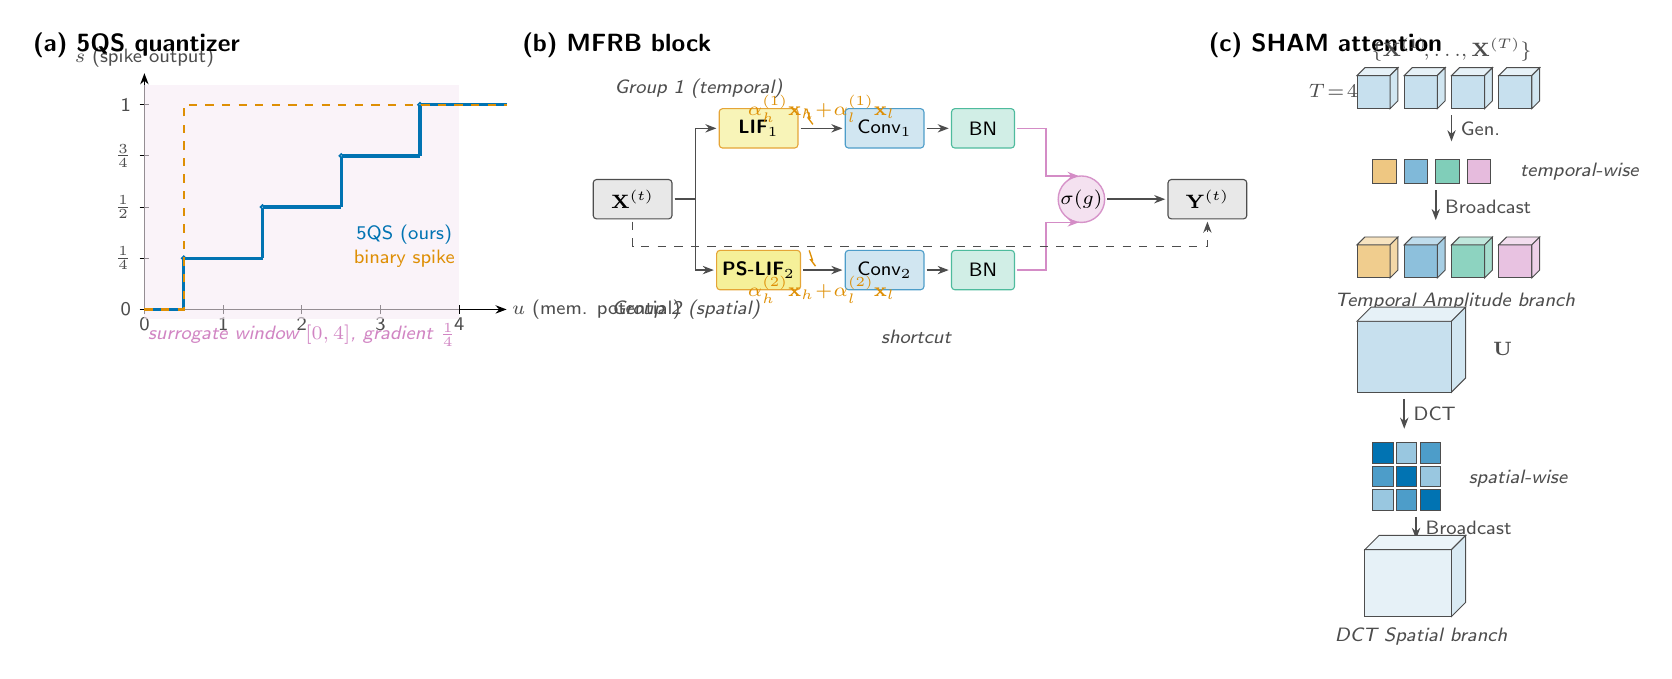
\begin{tikzpicture}

% =============================================================================
% Panel (a) — 5QS quantizer (5-level spike + surrogate gradient)
% =============================================================================
\begin{scope}[shift={(0,0)}]
  % Axes
  \draw[axis] (0, 0) -- (4.6, 0) node[right, label]{$u$ (mem. potential)};
  \draw[axis] (0, 0) -- (0, 3.0) node[above, label]{$s$ (spike output)};

  % Tick marks on x-axis (u = 0, 1, 2, 3, 4)
  \foreach \x in {0,1,2,3,4} {
    \draw (\x, -0.06) -- (\x, 0.06);
    \node[label, anchor=north] at (\x, -0.04) {\x};
  }

  % Tick marks on y-axis (s = 0, 1/4, 1/2, 3/4, 1)
  \foreach \y/\lbl in {0/0, 0.65/$\tfrac14$, 1.30/$\tfrac12$,
                       1.95/$\tfrac34$, 2.60/1} {
    \draw (-0.06, \y) -- (0.06, \y);
    \node[label, anchor=east] at (-0.10, \y) {\lbl};
  }

  % Surrogate gradient window (rectangular, [0, 4])
  \fill[cPurple!15, opacity=0.6]
    (0, -0.12) rectangle (4, 2.85);
  \node[label, text=cPurple!90, font=\sffamily\scriptsize\itshape]
    at (2, -0.32) {surrogate window $[0,4]$, gradient $\tfrac{1}{4}$};

  % 5QS step function (forward)
  \draw[line width=1.2pt, draw=cBlue]
    (0,    0)    -- (0.5,  0)
    (0.5,  0)    -- (0.5,  0.65)
    (0.5,  0.65) -- (1.5,  0.65)
    (1.5,  0.65) -- (1.5,  1.30)
    (1.5,  1.30) -- (2.5,  1.30)
    (2.5,  1.30) -- (2.5,  1.95)
    (2.5,  1.95) -- (3.5,  1.95)
    (3.5,  1.95) -- (3.5,  2.60)
    (3.5,  2.60) -- (4.6,  2.60);

  % Step transitions visualised as small open circles (right end open, left end closed)
  \foreach \x/\y in {0.5/0.65, 1.5/1.30, 2.5/1.95, 3.5/2.60} {
    \fill[white, draw=cBlue, line width=0.6pt] (\x, \y) circle (0.7pt);
  }

  % Binary spike comparison (dashed)
  \draw[line width=0.8pt, draw=cOrange, dashed]
    (0, 0) -- (0.5, 0) -- (0.5, 2.60) -- (4.6, 2.60);

  % Legend
  \node[label, text=cBlue]   at (3.3, 0.95) {5QS (ours)};
  \node[label, text=cOrange] at (3.3, 0.65) {binary spike};

  % Sub-panel label
  \node[panellbl] at (-0.1, 3.35) {(a) 5QS quantizer};
\end{scope}

% =============================================================================
% Panel (b) — MFRB block (dual-frequency residual)
% =============================================================================
\begin{scope}[shift={(6.2, 0)}]
  % Input
  \node[block, fill=cLight, minimum width=10mm] (xin) at (0, 1.4) {$\mathbf{X}^{(t)}$};

  % Group 1 — temporal LIF path (top)
  \node[lifblk] (lif1) at (1.6, 2.3) {LIF$_1$};
  \node[convblk, minimum width=10mm] (c1) at (3.2, 2.3) {Conv$_1$};
  \node[bnblk] (b1) at (4.45, 2.3) {BN};

  \draw[arrow] (xin.east) -- ++(0.3, 0) |- (lif1.west);
  \draw[arrow] (lif1) -- (c1);
  \draw[arrow] (c1) -- (b1);

  % Group 2 — spatial PixelShuffle path (bottom)
  \node[lifblk, fill=cYellow!50] (ps2) at (1.6, 0.5) {PS-LIF$_2$};
  \node[convblk, minimum width=10mm] (c2) at (3.2, 0.5) {Conv$_2$};
  \node[bnblk] (b2) at (4.45, 0.5) {BN};

  \draw[arrow] (xin.east) -- ++(0.3, 0) |- (ps2.west);
  \draw[arrow] (ps2) -- (c2);
  \draw[arrow] (c2) -- (b2);

  % High/low freq scale annotations on each path
  \node[label, text=cOrange, font=\sffamily\scriptsize] at (2.4, 2.55)
        {$\alpha_h^{(1)} \mathbf{x}_h \!+\! \alpha_l^{(1)} \mathbf{x}_l$};
  \node[label, text=cOrange, font=\sffamily\scriptsize] at (2.4, 0.25)
        {$\alpha_h^{(2)} \mathbf{x}_h \!+\! \alpha_l^{(2)} \mathbf{x}_l$};

  % Cross-scale gate (sigmoid) — multiplicative gate combining the two high-freq paths
  \node[gateblk] (gate) at (5.7, 1.4) {$\sigma(g)$};
  \draw[arrow, draw=cPurple!85, line width=0.5pt]
        (b1.east) -- ++(0.4, 0) |- (gate.north);
  \draw[arrow, draw=cPurple!85, line width=0.5pt]
        (b2.east) -- ++(0.4, 0) |- (gate.south);

  % Output
  \node[block, fill=cLight, minimum width=10mm] (yout) at (7.3, 1.4) {$\mathbf{Y}^{(t)}$};
  \draw[arrow] (gate.east) -- (yout.west);

  % Residual shortcut (curved, dashed)
  \draw[arrow, draw=cGray, dashed, line width=0.45pt]
        (xin.south) -- ++(0, -0.35) -| node[label, near end, right]{} (yout.south);
  \node[label, text=cGray, font=\sffamily\scriptsize\itshape]
        at (3.6, -0.35) {shortcut};

  % Spike symbols on LIF outputs (the lightning-bolt style)
  \pic at ($(lif1.east) + (1.5mm, 1.5mm)$) {spikemark};
  \pic at ($(ps2.east)  + (1.5mm, 1.5mm)$) {spikemark};

  % Group labels
  \node[label, text=cGray, font=\sffamily\scriptsize\itshape, anchor=west]
        at ($(lif1.west) + (-1.4, 0.50)$) {Group 1 (temporal)};
  \node[label, text=cGray, font=\sffamily\scriptsize\itshape, anchor=west]
        at ($(ps2.west)  + (-1.4, -0.50)$) {Group 2 (spatial)};

  \node[panellbl] at (-0.2, 3.35) {(b) MFRB block};
\end{scope}

% =============================================================================
% Panel (c) — SHAM attention (temporal amplitude + DCT spatial)
% =============================================================================
\begin{scope}[shift={(15.4, 0)}]
  \node[panellbl] at (-0.4, 3.35) {(c) SHAM attention};

  % --- Top: Temporal amplitude attention (T cubes -> 1-D temporal weights) ---
  % T = 4 input cubes
  \foreach \i in {0,1,2,3} {
    \pgfmathsetmacro{\cx}{0.6*\i}
    \draw[cube, fill=cBlue!22] (\cx, 2.55) rectangle ++(0.42, 0.42);
    \draw[cube, fill=cBlue!10]
      (\cx, 2.97) -- ++(0.10, 0.10) -- ++(0.42, 0) -- ++(-0.10, -0.10) -- cycle;
    \draw[cube, fill=cBlue!18]
      (\cx + 0.42, 2.55) -- ++(0.10, 0.10) -- ++(0, 0.42) -- ++(-0.10, -0.10) -- cycle;
  }
  \node[label, text=cGray, font=\sffamily\scriptsize] at (-0.30, 2.78) {$T\!=\!4$};
  \node[label, text=cGray, font=\sffamily\scriptsize\itshape] at (1.2, 3.30)
        {$\{\mathbf{X}^{(1)}\!,\ldots\!,\mathbf{X}^{(T)}\}$};

  % Generation arrow
  \draw[arrow] (1.2, 2.50) -- (1.2, 2.10);
  \node[label, anchor=west, font=\sffamily\scriptsize] at (1.25, 2.30) {Gen.};

  % 1-D temporal weights (4 colored small squares horizontally)
  \foreach \i/\c in {0/cOrange, 1/cBlue, 2/cGreen, 3/cPurple} {
    \pgfmathsetmacro{\cx}{0.4*\i + 0.2}
    \draw[cube, fill=\c!50] (\cx, 1.60) rectangle ++(0.30, 0.30);
  }
  \node[label, font=\sffamily\scriptsize\itshape, anchor=west]
        at (2.00, 1.75) {temporal-wise};

  % Broadcast arrow
  \draw[arrow] (1.0, 1.55) -- (1.0, 1.10);
  \node[label, anchor=west, font=\sffamily\scriptsize] at (1.05, 1.30) {Broadcast};

  % Output cubes (T tinted cubes, each colored uniformly per-time)
  \foreach \i/\c in {0/cOrange, 1/cBlue, 2/cGreen, 3/cPurple} {
    \pgfmathsetmacro{\cx}{0.6*\i}
    \draw[cube, fill=\c!45] (\cx, 0.40) rectangle ++(0.42, 0.42);
    \draw[cube, fill=\c!25]
      (\cx, 0.82) -- ++(0.10, 0.10) -- ++(0.42, 0) -- ++(-0.10, -0.10) -- cycle;
    \draw[cube, fill=\c!35]
      (\cx + 0.42, 0.40) -- ++(0.10, 0.10) -- ++(0, 0.42) -- ++(-0.10, -0.10) -- cycle;
  }

  % --- Bottom row label ---
  \node[label, text=cGray, font=\sffamily\scriptsize\itshape, anchor=west]
        at (-0.35, 0.10) {Temporal Amplitude branch};

  % --- Bottom: DCT Spatial attention ---
  \begin{scope}[shift={(0, -3.6)}]
    % Input cube U^{t,n}
    \draw[cube, fill=cBlue!22] (0, 2.55) rectangle ++(1.2, 0.9);
    \draw[cube, fill=cBlue!10]
      (0, 3.45) -- ++(0.18, 0.18) -- ++(1.2, 0) -- ++(-0.18, -0.18) -- cycle;
    \draw[cube, fill=cBlue!18]
      (1.2, 2.55) -- ++(0.18, 0.18) -- ++(0, 0.9) -- ++(-0.18, -0.18) -- cycle;
    \node[label, text=cGray, font=\sffamily\scriptsize\itshape]
          at (1.85, 3.10) {$\mathbf{U}$};

    % FFT/DCT generation arrow
    \draw[arrow] (0.6, 2.50) -- (0.6, 2.05);
    \node[label, anchor=west, font=\sffamily\scriptsize] at (0.65, 2.27) {DCT};

    % 2-D spatial weights (small grid of colored squares)
    \foreach \i in {0,1,2} {
      \foreach \j in {0,1,2} {
        \pgfmathsetmacro{\cx}{0.30 * \i + 0.20}
        \pgfmathsetmacro{\cy}{0.30 * \j + 1.05}
        \pgfmathtruncatemacro{\hue}{40 + 30 * Mod(\i + \j, 3)}
        \draw[cube, fill=cBlue!\hue] (\cx, \cy) rectangle ++(0.26, 0.26);
      }
    }
    \node[label, font=\sffamily\scriptsize\itshape, anchor=west]
          at (1.35, 1.45) {spatial-wise};

    % Broadcast
    \draw[arrow] (0.75, 1.0) -- (0.75, 0.65);
    \node[label, anchor=west, font=\sffamily\scriptsize] at (0.80, 0.83) {Broadcast};

    % Output cube tinted with attention
    \draw[cube, pattern={Lines[angle=45,distance=1.2pt,line width=0.3pt]},
          pattern color=cBlue!70, fill=cBlue!10]
        (0.1, -0.30) rectangle ++(1.1, 0.85);
    \draw[cube, fill=cBlue!8]
        (0.1, 0.55) -- ++(0.18, 0.18) -- ++(1.1, 0) -- ++(-0.18, -0.18) -- cycle;
    \draw[cube, fill=cBlue!15]
        (1.2, -0.30) -- ++(0.18, 0.18) -- ++(0, 0.85) -- ++(-0.18, -0.18) -- cycle;

    \node[label, text=cGray, font=\sffamily\scriptsize\itshape, anchor=west]
          at (-0.35, -0.55) {DCT Spatial branch};
  \end{scope}
\end{scope}

\end{tikzpicture}
\end{document}
